\documentclass{mcmthesis}
\mcmsetup{CTeX = true,
        tcn = 83451, problem = A,
        sheet = true, titleinsheet = true, keywordsinsheet = true,
        titlepage = false, abstract = false}
\usepackage{palatino}
\usepackage{graphicx}
\usepackage{url}
\usepackage{amsmath}
\usepackage{subfigure}
\usepackage{listings}
\title{ Multi-hop HF Propagating Model with a Fractal Geometry Based Ocean Surface}
\author{\small Team \# 83451}
\date{\today}
\begin{document}

\begin{abstract}

Today, radio waves play an important role in all fields, ranging from mobile phones and radios to satellite positioning. Shortwave communication in the sea is even more important. It is mainly spread by means of multiple reflections (multi-hop paths) of the sky wave between the ionosphere and the ground. Therefore, studying the multi-wave model has a very positive significance for the maritime communications.

In this paper, we will study the reflection between the ionosphere and sea surface in a multi-hop model. Then we make some reasonable suggestions for the terrestrial launch antennas and the maritime vessels to improve our communication quality. Our work is mainly steped as the flowing structure.

First, we will construct a high-frequency electromagnetic reflection model between the ocean surface \emph{(both of a turbulent surface and a calm one)} and the ionosphere. We also make some simplifications for the ionosphere and the ocean surface. As for generating a turbulent ocean surface, we use the \textbf{self-affine fractal Monte Carlo} method to construct the \textbf{Self-affine Gaussian spectrum} of the sea wave model. This fractal geometric method has been used to determine the roughness of a surface for many years.

Second, we calculate all the possible losses in the path, with the loss of each part basically in line with the actual value.

Then, we consider the changes of MUF during the day and the different seasons of the year, calculate the relationship between the first hop strength of calm and turbulent sea surface and the \textbf{maximum number of hops($N=2$)} of calm sea surface. After we applied this model to the terrain, we find the Extension of this model is very well.

Finally, considering the actual conditions of the sailing ships and the various factors of the shortwaves, we give a report on how to apply our model to the actual shortwave maritime communications.

\begin{keywords}
  Multi-hop model; Fractal structure; Rough surface; HF maritime communications
\end{keywords}
\end{abstract}
\maketitle

\tableofcontents
\newpage

\section{Introduction}

\subsection{Motivation}

On a sunny summer day, everyone wants to enjoy the pleasure of fishing on a yacht at sea. However, as we enter the deep ocean, chances are that our on-board HF(3-30MHz) receiver was unable to receive timely broadcast warnings of the coming bad weather from the Maritime Bureau, then our wonderful summer afternoon would be destroyed by the ensuing storm. Based on the current HF broadcast model, which consists a blind area, such stories will be staged on the sea for many years.

If we put this story apart, we will also find out that, in today's world, maritime activities are becoming more frequent. There is a need for seamless, efficient and reliable communications coverage in the area of high economic activity. We need a reliable ocean shortwave communication model to help us build a marine communications network.

\subsection{Problem Restatement}

In this work, we are required to solve the following problems:

\begin{itemize}
  \item Firstly, because we are required to discuss a communication model which needs to know specific physical information. So we will create a precise reflection model of the atmosphere (ionosphere layer) and ground (ocean surface).\\
  \item Secondly, applying our model, we need to stress out the differeces between the reflection on a turbulent sea and a calm ocean. Next, how many times can a shortwave reflects from the calm ocean should be discussed. \\
  \item Thirdly, considering the geometrical and physical common features of the earth's surface, we should apply our model to study of terrain surface.\\
  \item We will then optimize the model so that it allows us to test the situation where vessels traveling on turbulent sea waves communication properties. \\
  \item Finally, we should prepare a synopsis of our results suitable for publication as a short note in \emph{IEEE Communications Magazine}.
\end{itemize}

\section{General Assumptions}

    To simplify the real life situation, we will accept the following assumptions while we construct our models.

    \begin{itemize}

      \item a. We assume that the transmitting antenna radiates a particular frequency of spherical waves.

      \item b. According to the far propagating distance, the Earth-surface cannot be considered as a plane, which we always do to handle some daily problems. However, we can approximate the Earth  to a sphere with a radius of 640,000 km. In addition, \textbf{the ionosphere and the ocean are in concentric spheres}.

      \item c. Due to the facts that the light wave is one kind of \textbf{electromagnetic waves (EM waves)}, we assume that the ionosphere and the ocean's reflection of EM waves can be analyzed using the same method as \textbf{geometrical optics}.

      \item d. Suppose the temperature and pressure in the entire propagation space path are almost constant, which means we will ignore the loss of EM waves caused by flowing air or non-constant physical characters (especially the temperature and pressure).

      \item e. We will not justify the electromagnetic noise from the radio receiver. We will assume that the noise mainly comes from the atmosphere.

    \end{itemize}

    \subsection{ourwork}

\section{Notations}

    \begin{table}[h]
      \centering
        \begin{tabular}{|c|c|l|}

          \hline Notations & Definition & Unit \\
          \hline $E_{r}$ & How much energy may trasmit to the receiver & $dBm$ \\
          \hline $E_{g}$ & How much energy will be generated & $dBm$ \\
          \hline $G_{r}$ & The antennas gain of receiver & $dBi$ \\
          \hline $G_{g}$ & The antennas gain of generator & $dBi$ \\
          \hline $L_{total}$ & The total energy loss during the propagation & $dB$ \\
          \hline $L_{fspl}$ & The free space path loss & $dB$ \\
          \hline $L_{a}$ & The loss during passing the ionosphere layer & $dB$ \\
          \hline $L_{grd}$ & The loss during the reflection on the grond & $dB$ \\
          \hline $L_{addition}$ & Additional loss of the signal energy & $dB$ \\
          \hline $\theta$ & The emitter elevation angle & $degree$ \\
          \hline $\phi$ & The incident angle in the ionosphere & $degree$ \\
          \hline

        \end{tabular}
        \caption{Notations}
    		\label{tab:Notations}
    \end{table}



\section{High Frequency Electromagnetic Waves}
  \subsection{High Frequency Electromagnetic Waves (HF-EM waves).}

    The electromagnetic wave, in physics, refers to the wave of the electronic field, propagating through space-time, carrying electromagnetic radiant energy. Classically, we can just study one component of the electromagnetic wave to represent the physical state of the entire wave. And the EM waves can be described as:

      \begin{equation}\label{eq:EMW}
        E = A * \cos(\omega t + \phi_{0})
      \end{equation}
      Where: \\
      $E$ is represent the electric field strength; \\
      $\omega$ is the angular frequency;\\
      $t$ represents how much time has passed since the wave had been generated;\\
      $\phi_{0}$ is the initial phase of the wave.\\

      And for studying the physical properties and changes of electromagnetic fields, we introduce the classical Maxwell equations:


      \begin{equation}\label{eq:Maxwell_new}
      \left\{
      \begin{aligned} % \begin{eqnarray}好像也可以。
          \nabla \times \textbf{H}  &= \textbf{J} + \frac{\partial\textbf{D}}{\partial t}       \\
          \nabla \times \textbf{E}  &= -\frac{\partial\textbf{B}}{\partial t}       \\
          \nabla   \cdot  \textbf{B}  &= 0       \\
          \nabla   \cdot  \textbf{D}  &= \rho
      \end{aligned}
      \right.
      \end{equation}
      The mathematical notations in this Equationa are the same as the habitual use of physical formulas


      As we known, \textbf{high frequency (HF)} is the designation for the range of radio frequency EM waves between 3 and 30 megahertz (MHz). The most interesting and important property of this frequency band, is that it can be reflected in the ionosphere layer in the atmosphere - a method which named \emph{sky wave} or \emph{skip}. It is because that the ionized atoms in the atmosphere can interact with HF-EM waves to change its radiating path.\cite{HF_EM}

      If the sky wave which reflected to the Earth can be reflected again by the ground, a \emph{multi-hop propagation} model would be formed between the ionosphere and the Earth-surface(Figure ~\ref{fig:Multi_hop}). Depending on multi-hop propagation, the scope of the HF communications has been greatly enhenced.

      \begin{figure}[h]
      \centering
      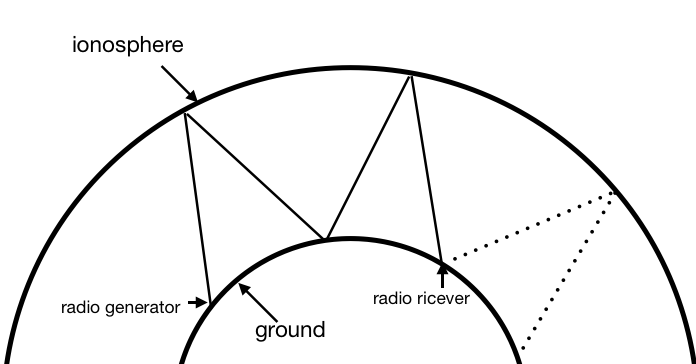
\includegraphics[scale=0.5]{Multi_hop}
      \caption{The Multi-hop propagation}
      \label{fig:Multi_hop}
      \end{figure}


  \subsection{HF-EM waves Propagation Model}

    Based on the modern physics common knowledge, HF-EM waves use the energy of the electromagnetic field to transmit information. So we can determine the signal strength by simply considering its enery. Especially in the radio-related applications, we usually use the unit known as decibel(\emph{dB}) to represent the energy relation of radio wave generating, transmitting and receiving. The decibel is a logarithmic unit used to express the ratio of the physical property to another, and may be used to describe a change in the value we discussed. Normally, the method of using decibel to describe the power quantity is:

      \begin{equation}\label{eq:power_dB}
        N|_{dB} = 10 \lg(\frac{P_{i}|_{W}}{P_{0}|_{W}})
      \end{equation}
      Where: \\
      $N$ represents the decibel figure we need to describe the ratio of the \textbf{current power} $P_{i}$ to the \textbf{initial power} $P_{0}$.\\

    In this paper, we will adopt this unit to describe the loss of the power in both of the ionosphere and ocean surface. Since we are solving a radio-related issue, to simplify our calculation, we will also use a unit named as dBm (power relative to 1 milliWatt) to measure the power of our EM waves. By the Equation \ref{eq:power_dB}, we get:

      \begin{equation}\label{eq:dBm_milliWatt}
        E |_{dBm} = 10 \lg(\frac{P_{i}|_{W}}{1 |_{mW} })
      \end{equation}

    Because we always use $W(Watt)$ as the power units, so the following Equation is commonly used:

      \begin{equation}\label{eq:dBm_Watt}
        E |_{dBm} = 30 + 10 \lg(\frac{P_{i}|_{W}}{1 |_{W} })
      \end{equation}

    In order to simulate the performance of multi-hop HF-EM waves between the ionosphere and the ocean, we need to measure the physical condition of it. As a EM wave, the essential property is how much energy it has. So the rate of its energy loss is the key factor in accessing a signal propagation process. Using the derived Equation \ref{eq:dBm_Watt} and the unit(dB), the rate of the energy loss can be calculate like this:

      \begin{equation}\label{eq:transmitting}
        E_{r} = E_{g} + G_{g} - L_{total} + G_{r}
      \end{equation}
      \emph{The characters we used has been discussed at Table \ref{tab:Notations}.}

    Since the units \emph{$dBi$} and \emph{$dBm$} has the same meaning of \emph{$dB$}, we can put them together in one formular. The physics meaning of this Equation is easy to understand. As the \emph{$dB$} represents the logarithmic ratio of two number, the multiplications between the initial energy values and the ratios of gain and attenuation can be simply replaced by addition and subtraction.

    From the requirement, which directly give us the energy intensity($P_{initial} = 100 W $) of the initial EM wave, we can assume that the initial wave energy containing both of the generating energy and the gain. Then, using Equation \ref{eq:dBm_Watt}, we can get this result:

      \begin{equation}\label{eq:E_initial}
        E_{initial} = E_{g} + G_{g} = 50 (dBm)
      \end{equation}

    As for the loss of the enery $L_{total}$, we assume the components of it are:

      \begin{equation}\label{eq:L_total}
        L_{total} = L_{fspl} + L_{a} + L_{grd} + L_{addition}
      \end{equation}

     In this section, we will only study on the free-space path loss ($L_{fspl}$). And the details of other sections of the enery loss will be analyzed later.

  \subsection{Signal-to-noise Ratio}
     \textbf{Signal-to-noise ratio} is a measure that compares the level of a desired signal to the level of background noise.

     \begin{equation}\label{eq:SNR}
     \left\{
     \begin{aligned}
         SNR &= \frac{P_{\text{signal}}}{P_\text{noise}} \\
         SNR|_{dB} &= P_{\text{signal}}|_{dB} - P_{\text{noise}}|_{dB}
     \end{aligned}
     \right.
     \end{equation}

  \subsection{Free-space Path Loss}
      The \textbf{free-space path loss(FSPL)}\cite{freespacepathloss} has been discussed for many years. FSPL can be used to calculate the signal strength loss when an EM wave travels over a line of sight path in free space. Based on the \emph{Assumption a} and exsting model of spherical waves in free space \emph{(between the ionosphere and the ground)}, we can draw the result of that:

        \begin{equation}\label{eq:FSPL_old}
          L_{fspl} = (\frac{4 \pi d f}{c})^{2}
        \end{equation}
        Where: \\
        $d$ is the distance of the receiver from the transmitter (metres)\\
        $f$ is the signal frequency (Hertz)\\
        $c$ is the speed of light in a vacuum (metres per second)\\

      If we use \emph{dB} as the unit, then we convert this formula to:

        \begin{equation}\label{eq:FSPL_applied}
          L_{fspl} = 20\log(d) + 20\log(f) + 32.44
        \end{equation}
        Where:\\
        $d$ is the distance of the receiver from the transmitter (km)\\
        $f$ is the signal frequency (MHz)\\

      \emph{Notice: the units we use in the Equation \ref{eq:FSPL_old} and Equation \ref{eq:FSPL_applied} are different. In the following Equations, except for special Notice, we will take the frequency unit as MHz}

      By applying this formular, the FSPL can be simply calculated if we have the value of free space distance and the frequency of our EM wave.

\section{The Ionosphere}

  \subsection{The Ionosphere Structure Model}
    The ionosphere is a shell of electrons and electrically charged atoms and molecules that surrounds the Earth, stretching from a height of about 50 km to more than 1,000 km. It exists primarily due to ultraviolet radiation from the Sun. Classically, ionosphere has four layers, which named D; E; F1 and F2 (from lower to higher), and each layer has its own unique physical property.\cite{davies1990ionospheric} Some basic information of the four layers is being displayed in Table \ref{tab: the ionosphere layers}.

        \begin{table}
          \centering
            \begin{tabular}{|l|l|l|}
            \hline
            Layers                  &Day & Night      \\ \hline
            F2 (lower than 500 km)  & The main reflection layer for HF waves & combine with F1          \\ \hline
            F1 (higher than 150 km) & Forming during day time       & combine with F2    \\ \hline
            E  (90 to 150 km)       & Absorb the HF waves (less than 10dB) & weaker than daytime          \\ \hline
            D  (60 to 90 km)        & Existing, and absorb HF waves &disappear  \\ \hline
            \end{tabular}
            \caption{The layers of ionosphere}
            \label{tab: the ionosphere layers}
        \end{table}

    Although there are many charged particles in the ionosphere that affect the propagation of HF-EM waves, the number of electrons in the ionosphere is much higher than that of other particles due to solar radiation. Therefore, we assume here that the sources which affect the physical properties of the ionosphere are mainly Electronic number density $N_{e}$.

    In order to describe the electromagnetic properties of the ionosphere, from Maxwell's Equations \ref{eq:Maxwell_new}, we need to know the dielectric constant in the ionosphere. From the previous study\cite{davies1990ionospheric}, we know:

      \begin{equation}\label{eq:relative_dielectric}
        \varepsilon_{r} = 1 - \frac{80.8 * N_{e} * 10^{6}}{f^{2}}
      \end{equation}
      where:\\
      $\varepsilon_{r}$ is the relative dielectric constant of the ionosphere;\\
      $f$ is the signal frequency (MHz) \\

    Since $\varepsilon_{r} = \frac{\varepsilon}{\varepsilon_{0}}$, and \textbf{electric susceptibility}$\chi = \varepsilon_{r} - 1$, then we draw the result:

      \begin{equation}\label{eq:chi}
        \chi = - \frac{80.8 * N_{e}}{f^{2}}
      \end{equation}




    We will discuss no more specific details of the ionosphere because we can easily get the values we need from previous studies. The data and parameters which we use to calculate the propagation process in the atmosphere comes from \emph{International Reference Ionosphere - IRI - 2007}\cite{NASAIonosphere}, one of the NASA's database.


  \subsection{'Skip' Model and Ionospheric Absorption Loss}

    As we discussed in the sections above, we have the Figrue ~\ref{fig:Multi_hop} to represent the HF-EM waves propagating model. In this section, we will determine some details of the HF-EM waves' propagating process in the upper atmosphere known as skay wave or 'skip'.

    In general, Since we can obtain the data and basic parameters of the ionosphere. Considering the differences between the four layers \emph{(especially the difference in $N_{e}$)} and its basic physical properties, and from the reference book\cite{davies1990ionospheric,terman1943radio} and Table \ref{tab: the ionosphere layers}, we will adopt this assumption to simplyfy our measurment:

    \begin{itemize}
      \item Assumption f. We assume that the main absorbtion of the HF-EM waves lies in the D-layer(about 100km) and reflection in the F2-layer(about 300km).
    \end{itemize}

    \begin{figure}[h]
    \centering
    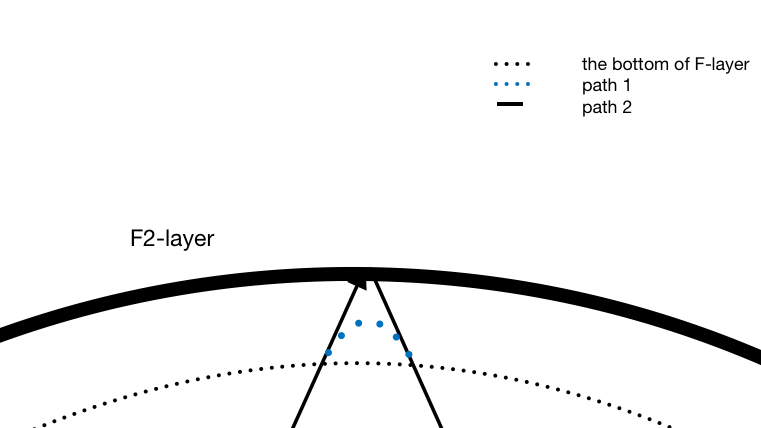
\includegraphics[scale=0.5]{PathinIonosphere}
    \caption{The different path in the ionosphere}
    \label{fig:PathinIonosphere}
    \end{figure}

    And if we consider the general nature of geometrical optics on this Assumption, then we can get such a simplified image(Figure ~\ref{fig:PathinIonosphere}). In the real world, the HF-EM wave's propagating path looks like a parabola (Figure X, \emph{path 1}), however, in our work, we simplyfy this kind of path to the basic form of specular reflection (\emph{path 2}). We took this simplification after making some estimations. First, the EM-wave absorption in the F-layer is first much smaller than absorption in the D-layer, the effect of the F-layer can be neglected in calculating the \textbf{ionospheric absorption} \emph{(which we will discuss in this section's following part)}. Second, if we consider the value of the free-space path loss($L_{fspl}$), the energy lost through \emph{path 1} and \emph{path 2} is negligible because the distance traveled in the ionosphere is much less than the height between the ground and the ionosphere.

    \textbf{Ionospheric absorption loss $L_{a}$} comes from the fact that, when the radio waves passes through, the electrons, ions and neutral molecules in the ionosphere will collide and generate heat in the electromagnetic field. In this process, the electric wave itself loses energy.

    Ionospheric absorption loss is related to the electron number density $N_{e}$, collision rate $v$, the intensity of geomagnetic field and the frequency of radio waves. However, it is difficult to accurately estimate the ionospheric parameters - $N_{e}$, $v$ and so on. Therefore, engineering calculations are often used semi-empirical formula for calculation and prediction\cite{terman1943radio}:

     \begin{equation}\label{eq:IonosphereLoss}
     \left\{
      \begin{aligned}
      L_{a} &= \frac{677.2}{(f + f_{H})^{1.98} + 10.2}\sum_{i = 1}^{n}\sec\phi_{i} \cdot I_{i}\\
      f_{H} &= 0.012333 \cdot \Phi + 0.892778
      \end{aligned}
      \right.
     \end{equation}
     where:\\
     $\phi$ is the incident angle at the ionosphere;\\
     $I$ is the absorbtion Index;\\
     $N$ refers to the total number of the hops;\\
     $i$ indicates the current number of hops;\\
     $\Phi$ Geographic Latitude of the position we discussed.

    Like the \emph{path 2} in Figure ~\ref{fig:PathinIonosphere}, the incident angle $\phi$ in the ionosphere can be calculate from the launch angle $\theta$ of the radio waves with some geometrical consideration in Figure ~\ref{fig:Multi_hop_angle}. We can get the result that:

    \begin{figure}[h]
    \centering
    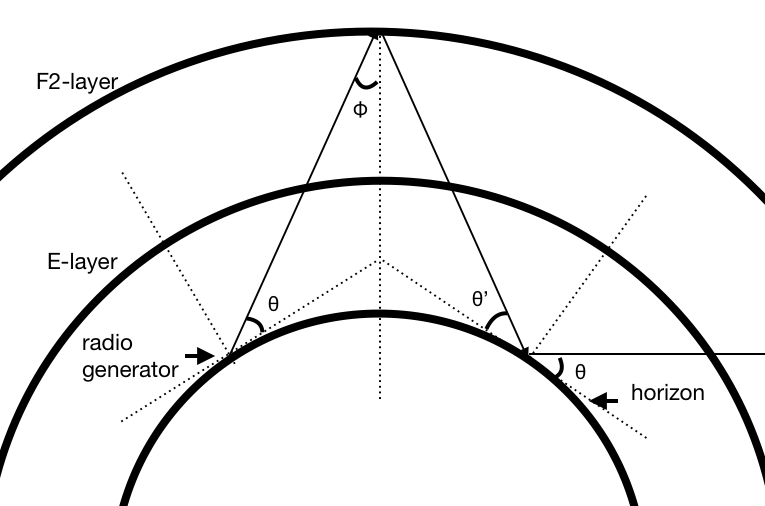
\includegraphics[scale=0.4]{Multi_hop_angle}
    \caption{The geometrical analysis of 'skip' }
    \label{fig:Multi_hop_angle}
    \end{figure}

    \begin{itemize}
      \item From the Figure ~\ref{fig:Multi_hop_angle}, we have $\theta = \theta'$. We will then conclude: the incident angles both at the ionosphere and ground maintain the same at every hops. We will use $\theta$ to represent the luanch angle and $\phi$ as the incident angle at the ionosphere. \\
      \item Considering the Earth's raduis $R_{earth}$ and the height of the F-layer $h_F$, the relationship between two angls is:

        \begin{equation}\label{eq:getPHI}
          \sin\phi = \frac{R_{earth}}{R_{earth} + h_{F}} * \sin(\theta + \frac{\pi}{2})
        \end{equation}

    \end{itemize}



    As for the absorbtion index, we have this result:

     \begin{equation}\label{eq:IonosphereAbsorbtionIndex}
       I = (1 + 0.037 R)(\cos0.881\chi)^{1.3}
     \end{equation}
     Where:\\
     $\chi$ is the electric susceptibility which we have calculated above;\\
     $R$ is the number of \textbf{Sun Spots} which we can get from previous work\cite{dayandyearTECchange};

     The parameters such as $N_{e}$ and $R$ involved in the formula can be obtained by means of ionospheric prediction and mapping. In this paper, we obtained these values of parameters from the NASA's Database.

\subsection{Maximum Usable Frequency}

    In radio transmission maximum usable frequency (MUF) is the highest radio frequency that can be used for transmission between two points via reflection from the ionosphere (skywave or 'skip' propagation) at a specified time, independent of transmitter power\cite{davies1990ionospheric}.

    \begin{equation}\label{MUF_def}
      f_{MUF} = \frac{ 9 \times \sqrt{N_e} }{\cos(\phi)}
    \end{equation}


\section{The Ocean}

  \subsection{Roughness Analysis Method}
    Since we are required to discuss the reflection on a turbulent ocean surface. The turbulent  we need a way to qualify a rough surface like this.

    In mathmatics, a \textbf{fractal} is an abstract object used to describe and simulate natually occuring objects. With this fractal.From the fractal idea, we can express any two-dimensional or high-dimensional image by concrete expressions. In recent years, \textbf{Fractal Geometry} has become a commonly used method to describe a rough surface\cite{lang2015hydraulic,shibuichi1998super}. Based on this method, we can eliminate the randomness of a rough surface and analyze its uniform characteristics.

    We will adapt the multifractal \textbf{detrended fluctuation analysis (MF-DFA)} method from \emph{JW Kantelhardt et al.2002}\cite{kantelhardt2002multifractal}. The detailed steps of this method are not repeated here. Its main idea is that:

    To analyze a rough surface, we usually use the \emph{Fast Fourier Transformation} to sample the surfaces' height. Use the fractal analysis of its parameters: range and variance. Which means we will divide the surface into many sections, and then consider the correlation of the samples in this section we determined. In each section $v$ (from $0$ to $N_s$), with \textbf{length $s$}, we will get an evaluating function $F^2(s,v)$. Using this function in each section, then average over all sections, we will get Equation \ref{eq:F_q} to get the $q$th order fluctuation function:

    \begin{equation}\label{eq:F_q}
      F_q(s) \triangleq (\frac{1}{N_s}\sum_{v=1}^{N_s}(F^2(s,v))^{q/2})^{1/q}
    \end{equation}

    The \textbf{roughness evluating function} $F_q(s)$ can be used to describe the surface of a part of the relevance. If we sampling the surface for many times, we can always get a statistical conclusion like this:

    \begin{equation}\label{eq:F_qq}
      F_q(s) \sim s^{H(q) + 1}
    \end{equation}
    Where:\\
    $q$ is a variable real number;\\
    $H$ refers to the Hurst Exponents.

    This conclusion suggests that the $F_q(s)$ itself is obey this distribution which determined by the $q$ and $H$. So these 2 figures are always used to justify the roughness of a surface.

  \subsection{Inverse Roughness Analysis Creation Method}

    If we start from the last step of this MF-DFA method, we may get a rough surface by setting a coherent length $s$, a index $q$, a Hurst Exponent $H$ and a hypothetical waveform function for each little section. So we will get a rough surface following these steps:

      \begin{itemize}
        \item We first need to set up a series of sampling points $n^2$; \\
        \item Then we will devide these points into several parts which we called \textbf{Coherent Sections}, which has $s^2$ points. Use the parameters ($q$, $H$) to give the roughness evluating function $F_q$ in each section. Since we just get the distribution $s^{H(q) + 1}$, we assume that the points we have in each section will obey $F_q(s)$ distribution; \\
        \item Then we combine the hypothetical \textbf{turbulent ocean waveform function $F_{wave}$ } and the $F_q(s)$. Let each point samples from this joint probability distribution; \\
        \item Do an Inverse Fast Fourier Transform for each point;\\
        \item Then we get the rough surface like the Figure ~\ref{fig:sample_ocean}.
      \end{itemize}

    Because our method basically obeys the general method of random sampling by using a computer, we can also call this method a fractal geometric method under the \textbf{Monte Carlo} method.

      \begin{figure*}[!t]
            \centering
            \subfigure[in 2-dimension] {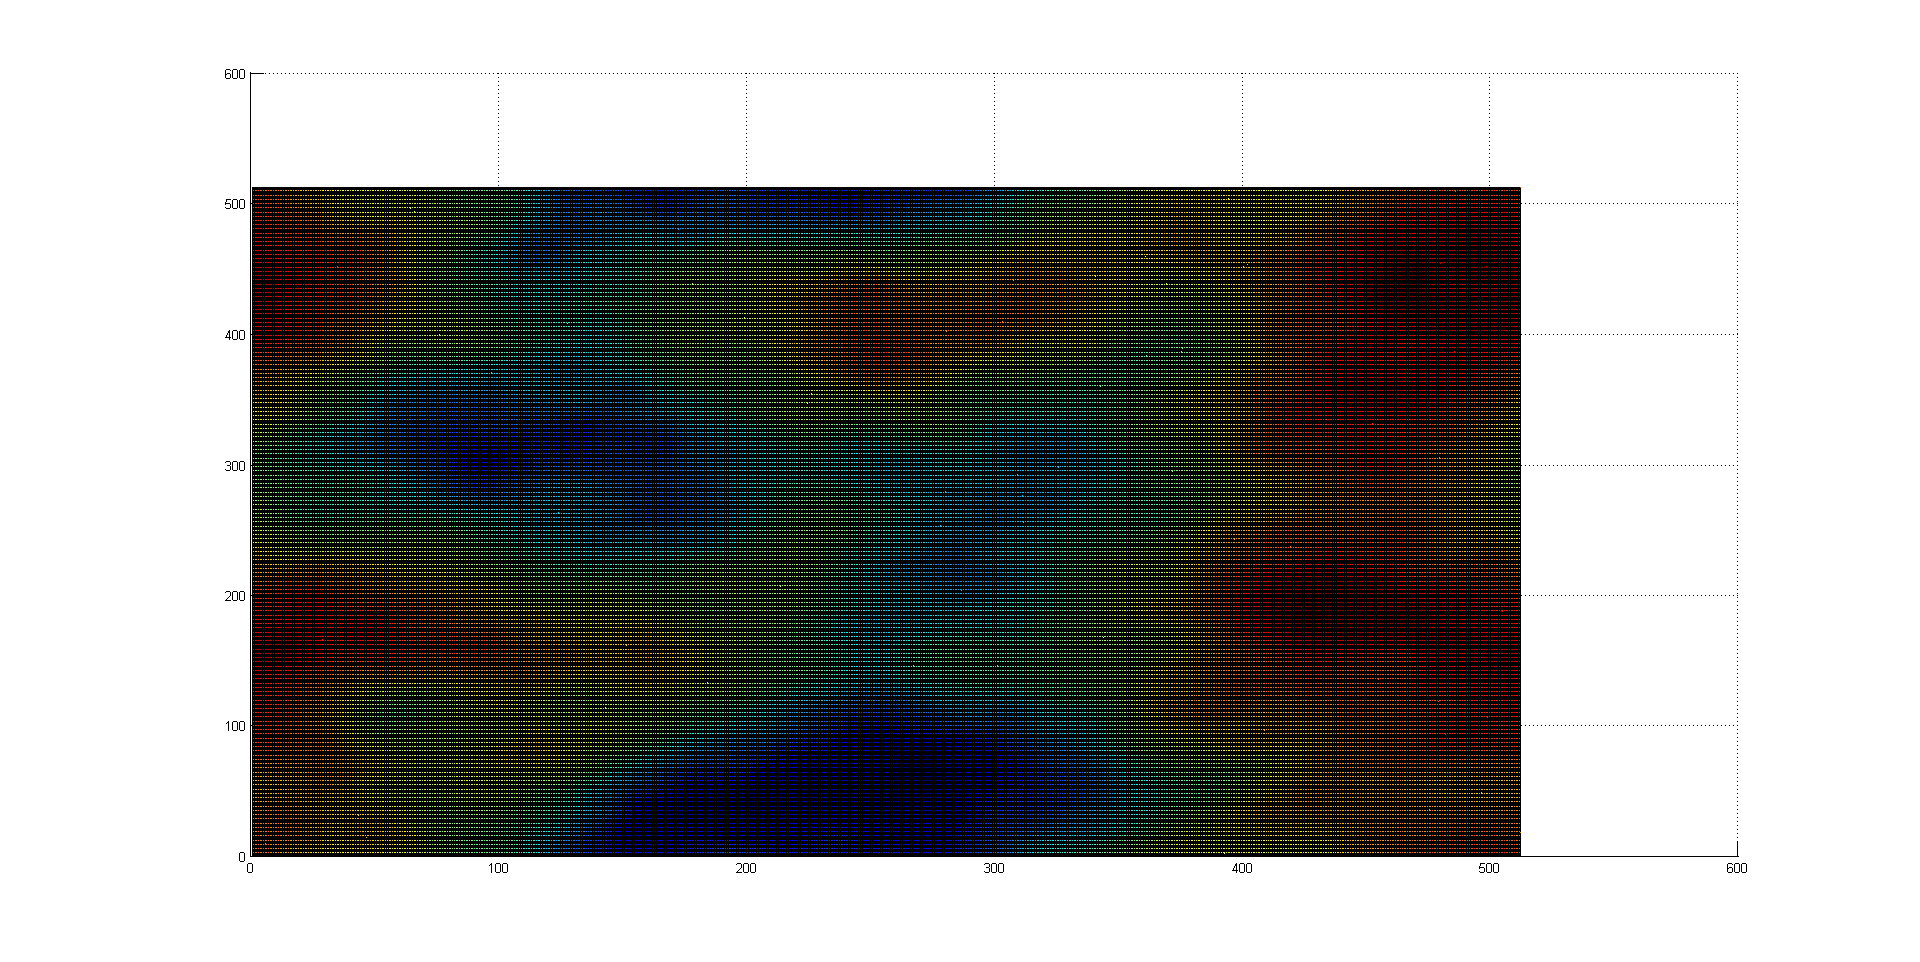
\includegraphics[scale=0.3]{2d-ocean}}
            \subfigure[in 3-dimension] {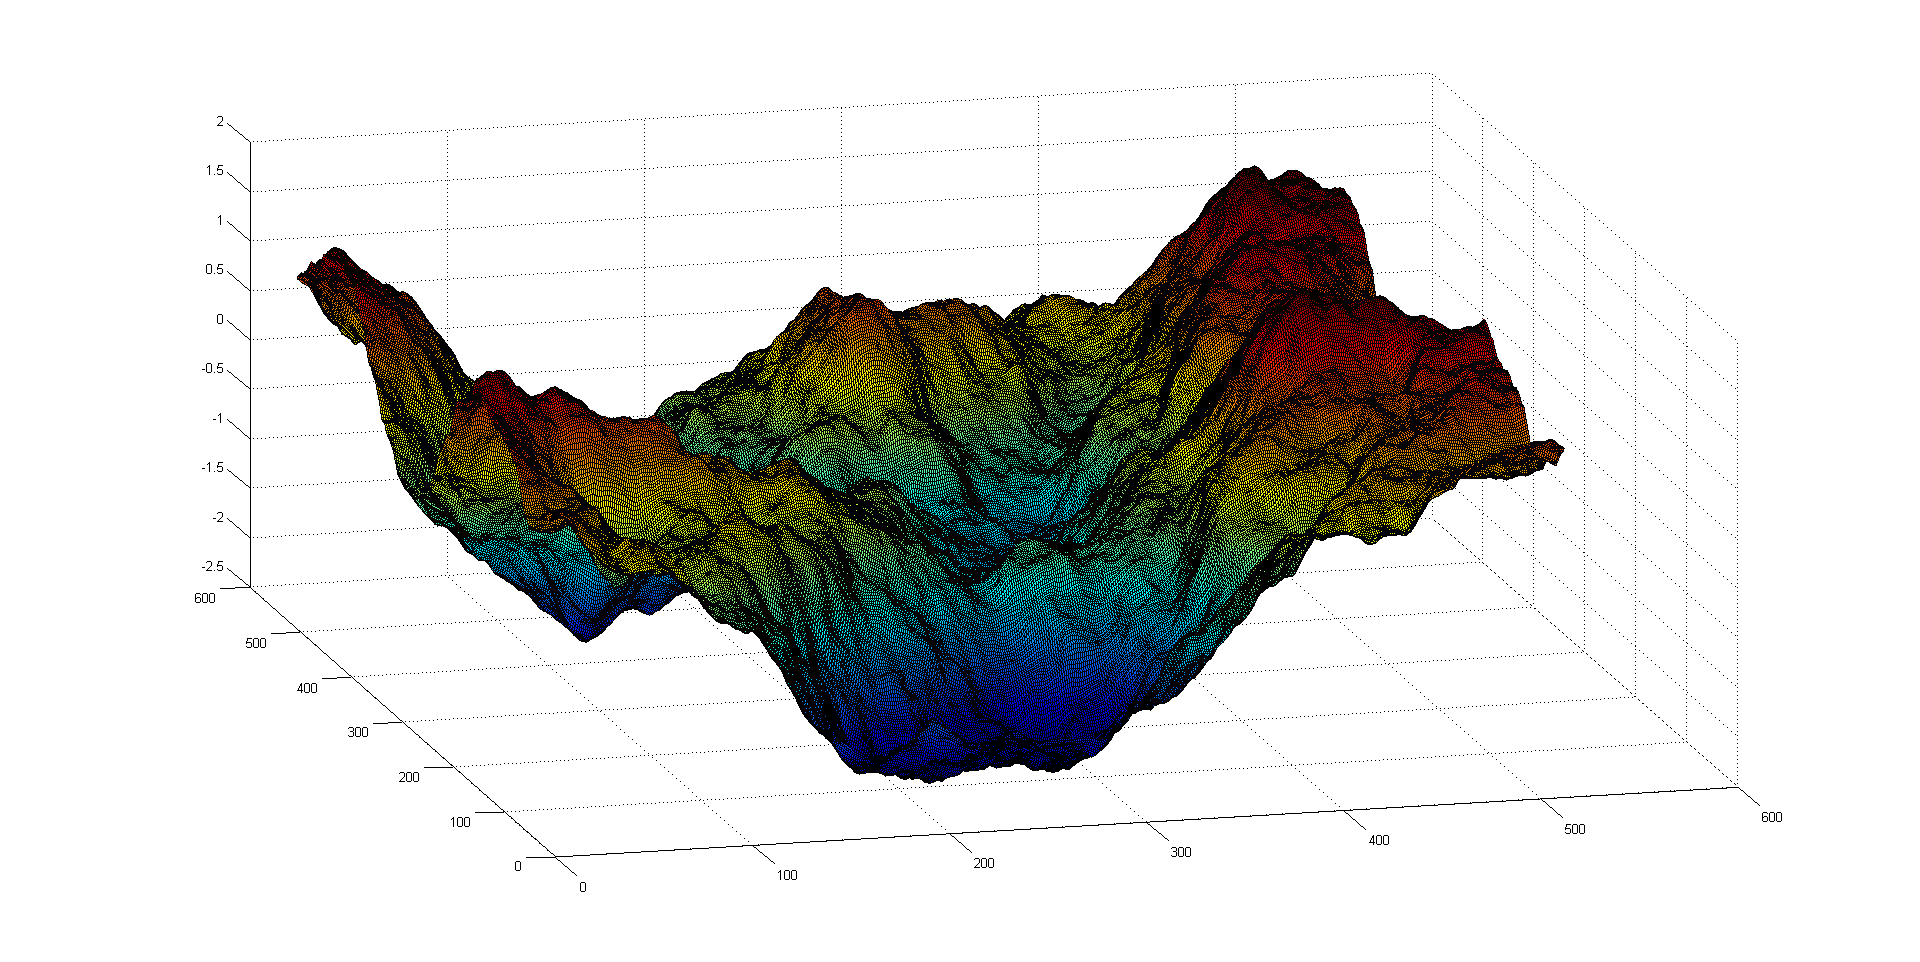
\includegraphics[scale=0.3]{3d-ocean}}
            \caption{A Sample of Creating a Turbulent Ocean Surface}
            \label{fig:sample_ocean}
      \end{figure*}

    \emph{Notice: For more details about our generating process of a rough surface, please check the \textbf{Appendix A}}.

    In addition, since $s$, $q$ and $H$ are used to define a surface correlation, there is no exact relationship of them. If we want to estimate a rough surface, then using 3 variables (one of which can be manually adjusted) will certainly yield a more accurate statistic estimation. But if we use this inverse method to create a rough surface, then changing one of them is enough to affect the roughness of a surface. Therefore, in practice, we fixed $s$ and $q$ and only use $H$ to control the roughness of the surface.

    To form a surface by using this process, we also need to define a \textbf{turbulent ocean waveform function $F_{wave}$}. Since we assumed that on a turbulent ocean surface, the wind would not affect its height, then gravity will be the only factor that affects the shape of the surface. For each point on the surface, we assume that the height of it obeys the Gaussian distribution:

    \begin{equation}\label{eq:Height_Gaussian}
      Height_{points} \sim N(\mu,\sigma^2)
    \end{equation}


  \subsection{Ground Reflection Loss}
    Since our task containing studying on the differences between rough and smooth surface, so we construct a general model for discussing the loss of the enery on the ground.

    \begin{figure}[h]
    \centering
    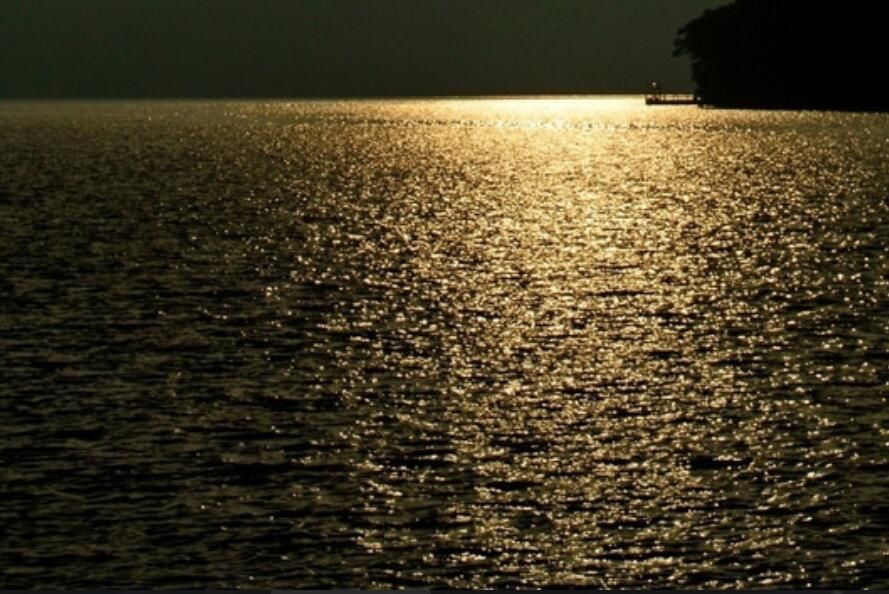
\includegraphics[scale=0.6]{waterface}
    \caption{A photo in a real world}
    \label{fig:waterface}
    \end{figure}

    Taken the Figure ~\ref{fig:waterface} into account, looking at a ocean surface at night, which points on the sea can be seen by our eyes or a camera len is an intersting question. If we take this physical image as the basis to consider the reflection of electromagnetic waves on the sea surface, we will give our answer:

    \begin{itemize}
      \item Assumption g. The overall reflection of the sea surface obeys the law of specular reflection (like the Figure ~\ref{fig:Multi_hop} \& ~\ref{fig:Multi_hop_angle}); \\
      \item Assumption h. Most of the light (EM waves) will be reflected from the \textbf{smooth part} of the rough surface. \\
    \end{itemize}

    Accepting these Assumptions, we will discuss the loss on the ground by the following Equation:

    \begin{equation}\label{eq:grd_L_total}
      L_{grd} = L_{plane} + L_{fresnel} + L_{mirror} + L_{visible}
    \end{equation}

    Or written in the form of multiplication by using Equation \ref{eq:power_dB}:

    \begin{equation}\label{eq:grd_R_Multiplication}
      R_{ground} = R_{plane} \times R_{fresnel} \times R_{mirror} \times R_{visible}
    \end{equation}

    We will discuss separately the components of the Equation \ref{eq:grd_L_total} \& \ref{eq:grd_R_Multiplication}.

    $R_{plane}$ explains the \emph{Assumption h}. So we need to define the smooth part on the surface. Since we can get many samples ($n^2$) on the surface, we will have the height field of the surface from these samples. Then we introduce gradient to measure the smoothness of a 2-dimension height field $G(x,y)$:

      \begin{equation}\label{eq:gradient}
        |\nabla G(x,y)| = \sqrt{(\frac{\partial G(x,y)}{\partial x})^2 + (\frac{\partial G(x,y)}{\partial y})^2}
      \end{equation}

    The gradient's model of a point shows the maximum height change in the field at this position. So we just need to define a maximum gradient $Grad_{max}$ a point may have to control its reflection:

      \begin{equation}\label{eq:R_plane}
        R_{plane}(\xi) =
        \begin{cases}
          1&\text{$|\nabla \xi| \leq |Grad_{max}|$}\\
          0&\text{$|\nabla \xi| > |Grad_{max}|$}
        \end{cases}
      \end{equation}
      This equation is generally formed like a $\delta$ function.

    $R_{fresnel}$ reflects the physical fact of reflection loss. We can use Maxwell's Equations \ref{eq:Maxwell_new} and electromagnetic wave propagation boundary conditions to derive this coefficient\cite{Hainan}.

      \begin{equation}\label{eq:R_Fesnel}
        R_{fresnel} = \frac{\varepsilon_s \cos(\theta) - \sqrt{\varepsilon_s - \sin^2(\theta)}}{\varepsilon_s \cos(\theta) + \sqrt{\varepsilon_s - \sin^2(\theta)}}
      \end{equation}

    The $R_{mirror}$ we adopt has been derived by \emph{Ament,1953}\cite{ament1953toward} and corrected by \emph{Beard,1961}\cite{beard1961coherent}.

    \begin{equation}\label{eq:R_mirror}
    \left\{
    \begin{aligned}
        R_{mirror} &= exp(- P_s) B_{1th}(P_s) \\
        P_s &= 2 \times (\frac{2\pi h_{rms} \cos(\theta)}{\lambda})
    \end{aligned}
    \right.
    \end{equation}
    Where:\\
    $B_{1th}$ represents the First-order Bessel function.\\

    As for the $R_{visible}$, we consider the fact that on the turbulent ocean surface, the height of the waves would changed rapidly. Like the situation in Figure ~\ref{fig:visible}, chances are some waves would be shadowed by the latter. So we added a probability coefficient to consider if it would be blocked by waves. Since we generally assume that the height of the ocean wave obey the Gaussian distribution (Equation \ref{eq:Height_Gaussian}), so we have:

    \begin{equation}\label{eq:R_visible}
      R_{visible} = \lim_{N \to \infty} \prod_{i=1}^N \int_{h(x)}^{\infty} \frac{f(h(x),h_0)}{f(h_0)}d\xi
    \end{equation}
    Where:\\
    $f$ is the first- or second-order Gaussian distribution density function;\\
    $h_{0}$ represents the height of the reflecting point and $h(x)$ for the point at the distance $x$.

    We believe that the wave height spectra in each of our fractal structures (each single sections) do not obscure the other, whereas the wave spectra in different fractal structures are not correlated. Therefore, each occlusion we calculate here is based on each individual fractal structure, so here we make the two parameters in the second-order Gaussian distribution irrelevant. Which means we can change the second-order Gaussian to a multiplication of 2 first-order one in Equation \ref{eq:R_visible} to calculate the $R_{visible}$.

    \begin{figure}[h]
      \centering
      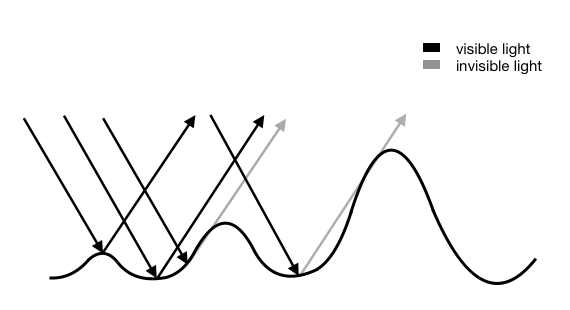
\includegraphics[scale=0.5]{Visible}
      \caption{Some EM waves would be shadowed by the following ocean wave}
      \label{fig:visible}
    \end{figure}

    Now that we have defined the method of calculating every partial loss in the HF-EM wave propagation path, we will test our model in the next few sections.

\section{Multi-hop HFEW Propagation Model}

    Based on the aforementioned ionospheric propagation model and ocean surface reflection model, we give the final multi-hop HF-EM wave model. The core of the mathematical model is to determine the energy loss by Equation \ref{eq:transmitting} \& \ref{eq:L_total}. Due to the simplification and assumptions of the model, we think that in addition to the energy losses we have already considered, other losses are not counted. So we will use this formular.

    \begin{equation}\label{eq:L_finaluse}
    \left\{
    \begin{aligned}
        E_{r} &= E_{g} + G_{g} - L_{total} + G_{r} \\
        L_{total} &= L_{fspl} + L_{a} + L_{grd} \\
        E_{initial} &= E_{g} + G_{g}
    \end{aligned}
    \right.
    \end{equation}

    Since we have defined the loss of each part in

    \subsection{Single-hop + Ocean Model}

      For simplify our Single-hop + ocean HF-EM wave transmission is a part of the multi-hop one, which has been shown in Figure ~\ref{fig:Multi_hop}. It includes two free-space path losses from the ground to the ionosphere and two losses by passing through the E-layer. The losses on a turbulent ocean surface also need to be considered.

      \begin{figure}[h]
      \centering
      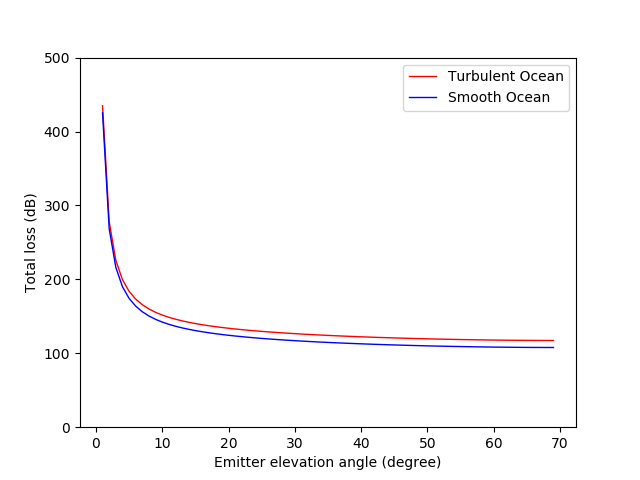
\includegraphics[scale=0.6]{Q1_10MHz}
      \caption{Comparison of 10 MHz HF-EM waves on turbulent ocean and smooth sea surface reflections}
      \label{fig:Multi_hop}
      \end{figure}

    \subsection{Multi-hop Propagation Model}

      After we have calculated a single hop, we can naturally extend this approach to multi-hop scenarios. Applying our geometric findings and previous analysis, we draw the result as:

      \begin{figure*}[!t]
      \centering
      \subfigure[N=2] {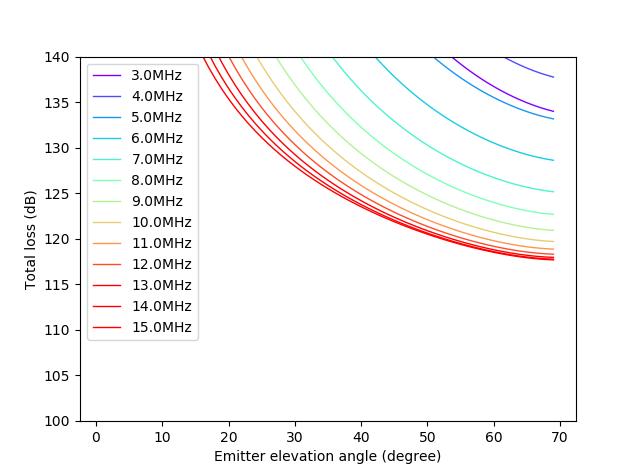
\includegraphics[scale=0.45]{Q1_N2}}
      \subfigure[N=3] {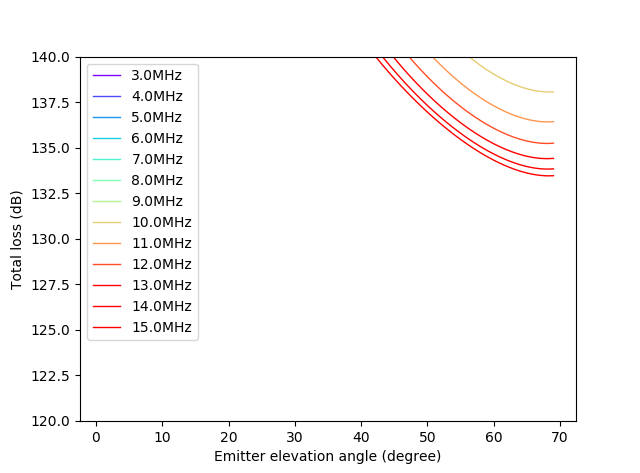
\includegraphics[scale=0.45]{Q1_N3}}
      \caption{ Multi-hop scenarios }
      \label{fig:Multi_hop_sc}
      \end{figure*}

      We assume that the loss below $130dB$ can meet the requirements of SNR($\ge 10$, assuming that the Noise is about $-80dB$). In this Figure, we can determine that the waves can not pass to the 2nd hop if its frequency is less than $6MHz$. And no wave can pass to the 3rd hop ($N = 3, loss < 130dB$).

    \subsection{The Extension of the Propagation Model}

      Next we apply this model to a mountainous terrain, where the main difference with the ocean surface is that there root mean square heights. For rough terrain, we set the root mean square height to 40 and 80 metres. Then we have the result:

      \begin{figure*}[!t]
      \centering
      \subfigure[hrm = 40] {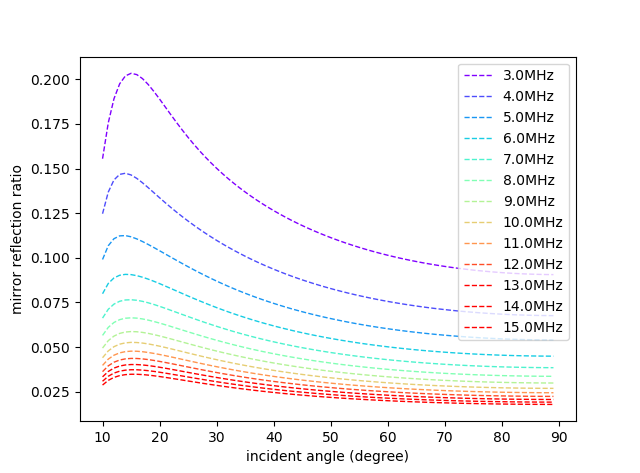
\includegraphics[scale=0.45]{Mon40}}
      \subfigure[hrm = 80] {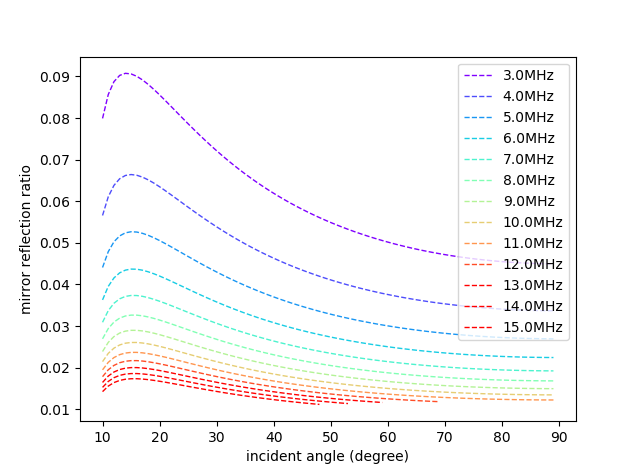
\includegraphics[scale=0.45]{Mon80}}
      \caption{ The mountainous terrain}
      \label{fig:mountainous}
      \end{figure*}

      In this Figure, We use reflectivity as the vertical axis, because we assume that the rest of the ground loss does not affect the static mountain surface.

      \begin{figure}[h]
      \centering
      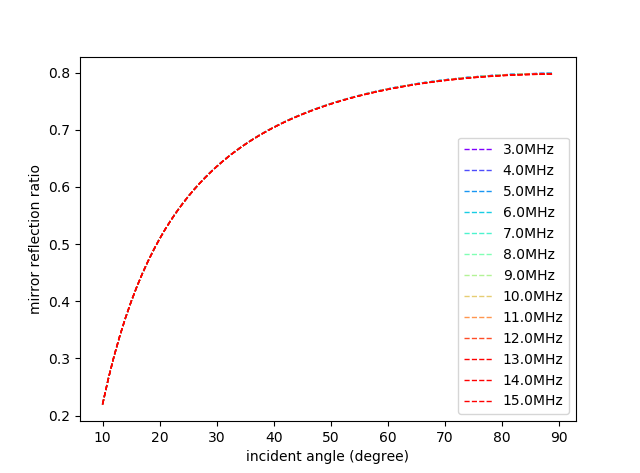
\includegraphics[scale=0.6]{Mon1}
      \caption{Smooth terrain}
      \label{fig:S_T}
      \end{figure}

      On the terrain, the reflection coefficients we find are orders of magnitude difference (roughly 1 order of magnitude) between rough and smooth surfaces(Figure ~\ref{fig:mountainous} \& ~\ref{fig:S_T}). If we want to add the influence of vegetation, the electromagnetic waves will be completely absorbed.

\section{Consider for Receivers}

      We all know that sailing ships need to rely on radio transmission to locate and receive weather reports and carry out other communication activities. While in this process, shortwave is the most commonly used in maritime communications. Therefore, our ocean HF-EM wave reflection model must start from the practical application and take the receiver on the ship into account.

      Vessels keep a certain speed on the ocean, and we need to ensure that the ships are always in communication. Therefore, we need to calculate the shortest and longest distance the skywave can cover. Then we will determine the best communication frequency for each distance at each place \& time.

      In addition, the ships on the turbulent ocean will sway, but when the transmission distance is far, the swaying of the ship has less effect on the signal reception. So we will not consider this kind of effect.


      \begin{figure}[h]
      \centering
      \includegraphics[scale=0.6]{Sample}
      \caption{Without considering MUF, we have this sample}
      \label{fig:Sample}
      \end{figure}

      In the Sample Figure ~\ref{fig:Sample}, the vertical axis is the total energy loss and the horizontal axis is the distance from the shore. In the picture we can see that there are 3 groups of lines separated from each other, from top to bottom respectively from 1-hop, 2-hops and 3-hops.

      To determine which frequency we suggests, we draw a series of figures in \emph{Appendix B}, just like the Sample Figure ~\ref{fig:Sample}. In addition, Considering the MUF change in a day, we remove the lines which is bigger than the \textbf{MUF}\ref{tab: MUF in HAWAII}. Just as we assumed earlier, the results we have are meant to describe a beautiful summer day in the \emph{Hawaii} district.

      \begin{table}[]
          \centering
          \caption{The change of the MUF in a day}
          \label{tab: MUF in HAWAII}
          \begin{tabular}{|l|l|}
          \hline
          the hours of a day & MUF(MHz) \\ \hline
          0-4                & 3.6572   \\ \hline
          4-8                & 7.4735   \\ \hline
          8-12               & 9.1551   \\ \hline
          12-16              & 11.7928  \\ \hline
          12-20              & 7.3326   \\ \hline
          20-24              & 4.6306   \\ \hline
          \end{tabular}
      \end{table}

      For a user, to Judge which frequency he needs at a certain distance, he only need to find the corresponding value of the line with the least energy loss (upper ones in the picture) from the figure. As a result, we find that radio stations transmitting different HF waves in a time range of 0-70$degree$ can receive signals more stably within 3000km of offshore as long as they patiently tune frequency from high frequency.

\section{Conclusion}
  \subsection{Strengths}
  \begin{itemize}
    \item We consider several important parameters influencing our model in detail and the influence of the parameter variation on the model is analyzed;\\
    \item The ocean wave model is based on the idea of fractal, which is in good agreement with the actual ocean wave conditio;\\
    \item The recommendations given for the frequencies required for reception of sky-wave signals by vessels at sea are of great help to the practical situation and have guiding significance for actual maritime communications. And our method can be easily adopted by people who need it.
  \end{itemize}

  \subsection{Weaknesses}
    \begin{itemize}
      \item The calculation of the sky-wave loss does not take into account latitude variations. In addition, the ionospheres' parameters we set are still relatively static and give rise to certain errors;\\
      \item There is a certain gap between the result and the previous result;\\
      \item There is no exact numerical value for the frequency list given to a vessel at sea nor the model of ship sway at sea. Since the method we used to generate rough surfaces by sampling from a distribution requires ample time to generate a large number of samples, but due to the limited time we cannot get a precise suggestion frequency as we expected;\\
      \item Because we use the position of $Hawaii$ in our analyze, the result we have for the \emph{IEEE Communications Magazine} may not suitable for other position.
    \end{itemize}

\newpage
\section{Synopsis to the \emph{IEEE Communications Magazine}}

\textbf{Abstract:}

  In this paper, we studied the multi-hop model of HF waves propagation. The key point is to take full account of the randomness of the ocean condition, and creating a rough ocean surface. We simulated and statistically analyzed the reflections, counting the loss of sea reflections and other possible aspect in the path. Finally, we provide a theoretical reference for maritime communications.

  As for the mathematical models, considering the physics fact of HF waves propagation, we have established a multi-hop HF waves propagation model, including the ionospheric reflection model, the turbulence and calm sea reflection model and distance-loss function to predict the ship's communication status

  When creating an ionospheric reflection model, we think that it is very difficult to obtain the physical parameters of the ionosphere in a specific and timely manner, and the model needs to be simplified. In this model, we equate the layered refraction of electromagnetic waves with a specular reflection of a suitable height. In addition, the ionospheric changes with the diurnal and seasonal changes will also be reflected in the MUF changes. As for the HF waves ionospheric loss and free space loss in the academic community have a more uniform method of calculation, we will not repeat them here.

  When we establish the sea surface reflection model, we think that the state of the water surface needs to be in accordance with the complex physical equations and there is a great randomness. Moreover, the \textbf{turbulence problem} is the most complex field in fluid mechanics. To complete a model that can quickly obtain approximate solutions, we need to find a path to extract the trunk of the problem and use as few parameters as possible to describe the sea state. We used a \textbf{self-affine fractal Monte Carlo method} to establish a sea-wave model that eventually decided to use the root-mean-square height and the fractal index. The wave distribution in our model fits the \textbf{Gaussian distribution} in the gravitational field, and then replenishes the water surface detail through the fractal structure, making it rough and simulating turbulence disturbing the water surface. We take a model with a certain area and the slope is extremely small. In each little section, we determine the reflection is similar to specular reflection, combined with the Fresnel formula. Applying the Monte Carlo method, we can calculate the energy loss on it.

  Multi-hop model also need to consider the description of the ship's position information, the most common spherical coordinates. After consideration, we think the use of spherical coordinate descriptions will complicate the issue since the location and distribution of the stations are uncertain. Finally, we get a simple parameter by analyzing the distance, angles and the transmission loss.

  In the design of the base station, we find that the most important parameters are the angle of the transmitted signal and the signal frequency. After preliminary statistics based on the above model, we found that radio stations transmitting different HFwaves in a time range of 0-70$degree$ can receive signals more stably within 3000km of offshore as long as they patiently tune frequency from high frequency.

  To sum up, our model is a useful and developmental model based on formula calculation and Monte-Carlo method to quickly calculate a radio frequency scheme that can communicate with vessels and to message the crew. Of course, we encountered some problems due to time constraints and obscure data. For example, we did not consider the position and other properties of a ship, especially its latitude. The calculated ionospheric scattering loss was not satisfactory. If we get more data and time, these problems can be solved. Hope the crew will always be safe.




\newpage
% \begin{thebibliography}{99}
%
%     \bibitem{1} D.~E. KNUTH   The \TeX{}book  the American
%     Mathematical Society and Addison-Wesley
%     Publishing Company , 1984-1986.
%     \bibitem{2}Lamport, Leslie,  \LaTeX{}: `` A Document Preparation System '',
%     Addison-Wesley Publishing Company, 1986.
%     \bibitem{3}\url{http://www.latexstudio.net/}
%     \bibitem{4}\url{http://www.chinatex.org/}
%
% \end{thebibliography}

\bibliographystyle{plain}
\bibliography{bib_83451}

\newpage
\begin{appendices}

  \section{The Generation Programmes}

    Here are simulation programmes we used in our model as follow.\\
    To generate a turbulent ocean surface,
    \textbf{\textcolor[rgb]{0.98,0.00,0.00}{Input Python source:}}

\lstset{language = Python}
\begin{lstlisting}
    import numpy as np
    import surface as sf
    def self_affine(saparams, power_of_two, seed=None):
        np.random.seed(seed)
        if saparams.lambda_0 is None :
        	lambda_0 = 1
        else:
        	lambda_0 = saparams.lambda_0
       	if saparams.lambda_1 is None :
       		lambda_1 = sys.maxsize
       	else:
       		lambda_1 = saparams.lambda_1
        N, L = 2**power_of_two, saparams.dimensions[0]
        power = -(saparams.hurst + 1.0)
        f_L = 1.0 / N
        f_0, f_1 = f_L * lambda_0, f_L * lambda_1
        A = np.zeros((N, N), dtype=complex)
        center = int(N / 2)

        rand_norm_1, rand_norm_2 = np.random.randn(center + 1, center + 1), np.random.randn(center + 1, center + 1)
        rand_unif_1, rand_unif_2 = np.random.rand(center + 1, center + 1), np.random.rand(center + 1, center + 1)
        for i in range(int(N / 2 + 1)):
            for j in range(int(N / 2 + 1)):
                phase = 2.0 * np.pi * rand_unif_1[i, j]
                rad = 0.0
                f = np.sqrt((float(i) / N)**2 + (float(j) / N)**2)
                if i != 0 or j != 0:
                    f = f if f > f_0 else f_0
                    rad = rand_norm_1[i, j] * f**power
                if f > f_1:
                    rad, phase = 0.0, 0.0
                A[i, j] = rad * np.cos(phase) + rad * np.sin(phase) * 1j
                i0 = 0 if i == 0 else N - i
                j0 = 0 if j == 0 else N - j
                A[i0, j0] = rad * np.cos(phase) - rad * np.sin(phase) * 1j
        A[center, 0] = A[center, 0].real + 0j
        A[0, center] = A[0, center].real + 0j
        A[center, center] = A[center, center].real + 0j

        for i in range(1, center):
            for j in range(1, center):
                phase = 2.0 * np.pi * rand_unif_2[i, j]
                f = np.sqrt((float(i) / N)**2 + (float(j) / N)**2)
                f = f if f > f_0 else f_0   # hi pass --> f_0
                rad = rand_norm_2[i, j] * f**power
                if f > f_1:                 # lo pass --> f_1
                    rad, phase = 0., 0.
                A[i, N - j] = rad * np.cos(phase) + rad * np.sin(phase) * 1j
                A[N - i, j] = rad * np.cos(phase) - rad * np.sin(phase) * 1j

        H = np.real(np.fft.ifft2((A)))
        s = sf.Surface(H, L / float(N))
        s = sf.scale_to_rms(s, saparams.hrms)
        s = sf.shift_to_zero_mean(s)
        return s
\end{lstlisting}

  \newpage
  \section{The Result for Hawaii}

        \begin{figure*}[ht]
        \centering
        \subfigure[00:00 to 04:00] {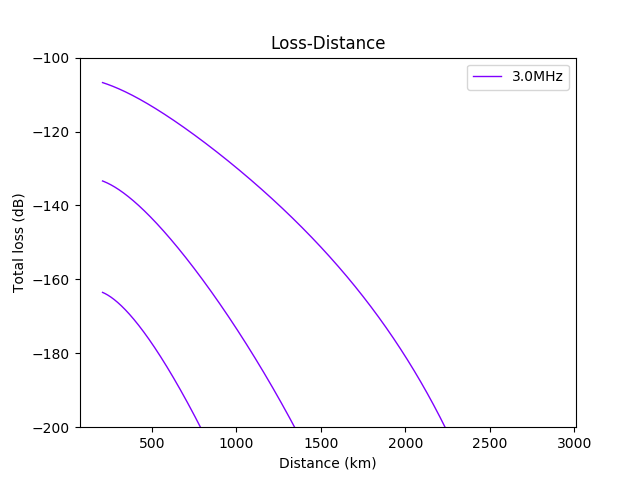
\includegraphics[scale=0.43]{mirro4}}
        \subfigure[04:00 to 08:00] {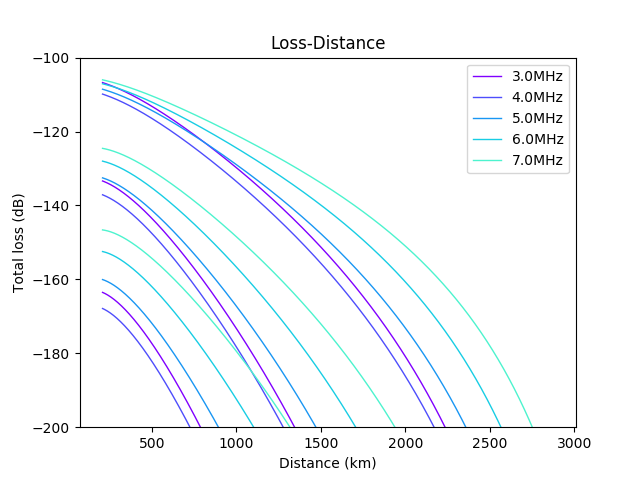
\includegraphics[scale=0.43]{mirro8}}
        \subfigure[08:00 to 12:00] {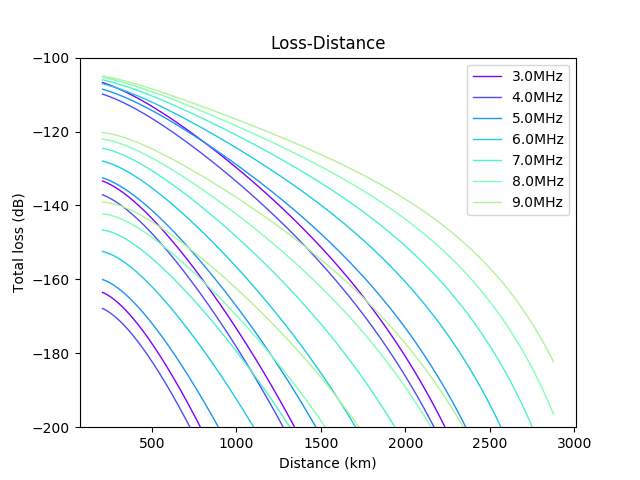
\includegraphics[scale=0.43]{mirro12}}
        \subfigure[12:00 to 16:00] {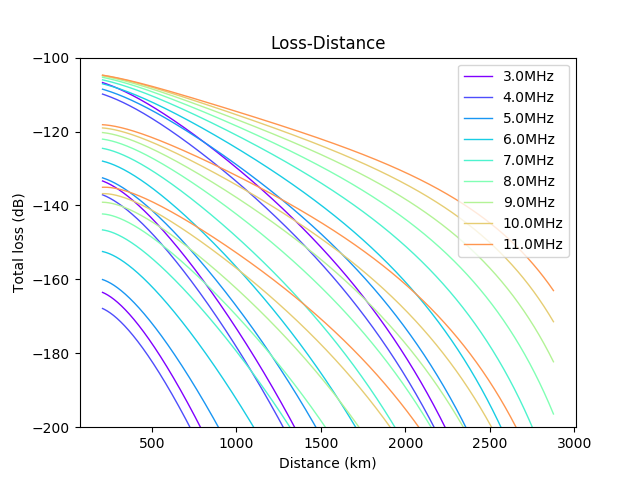
\includegraphics[scale=0.43]{mirro16}}
        \subfigure[16:00 to 20:00] {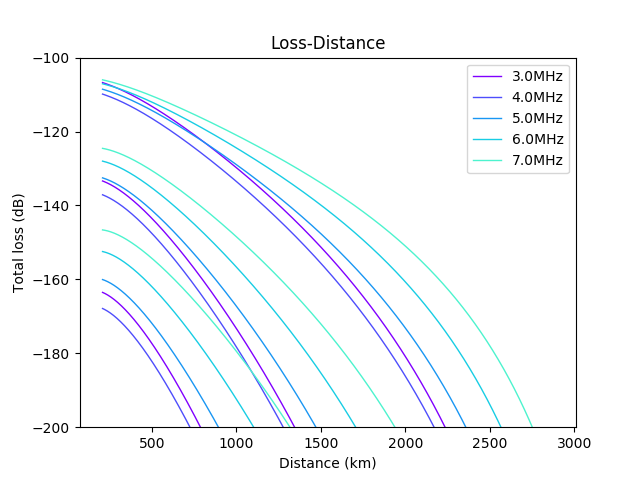
\includegraphics[scale=0.43]{mirro20}}
        \subfigure[20:00 to 24:00] {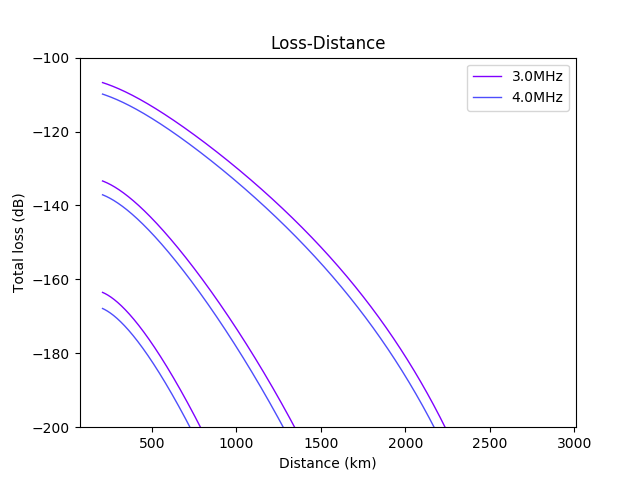
\includegraphics[scale=0.43]{mirro24}}
        \caption{ Loss - Distance (results for $Hwaii$)}
        \label{fig:LD}
        \end{figure*}

\end{appendices}



\end{document}
